% !Mode:: "TeX:UTF-8"

\chapter{测试向量压缩}

集成电路的发展日新月异,导致体积急剧减小的芯片上集成的晶体管数目却迅速增加,测试芯片需要的巨大测试数据集不仅提高了测试功耗,更增加了测试时间以及存储开销。数据压缩可以有效地解决上述问题。本章首先讲述电路可测性基础理论,然后就编码压缩方法、非编码压缩方法以及拆分压缩做进一步阐述。

\section{测试压缩原理}

测试压缩的主要目的在于减少测试数据量、降低测试时间以及节约最终的芯片制造成本。测试数据压缩可以采用多种方式,其目的均是为了降低原测试集中的比特位。当前比较常用的素具压缩算法有基于编码的数据压缩算法,基于线性扫描的数据压缩算法以及基于拆分测试集的数据压缩算法。

测试数据压缩有别于视频压缩,视频压缩属于有损压缩,可以丢弃残差集。当丢弃部分数据之后,并不会有损人们的视觉或者听觉效果。测试数据压缩属于无损压缩,压缩之后的数据需要被无差错地还原。测试集由0、1以及$X$位(无关位)组成,$X$位的产生和自动生成算法有关,测试集中具有较多的无关位,部分电路测试集甚至可达80\%以上。在测试压缩中,$X$根据特定的场景被任意地填充为0 或1,压缩率往往随着的无关位的增加而提高。本文主要针对测试激励进行相关压缩算法的研究,常见的测试激励压缩方法有广播扫描、编码压缩以及线性解压缩。 在测试响应压缩领域也有很多压缩方法,常用的有奇偶校验、特征分析等压缩方法。其中通过线性反馈移位寄存器(LFSR)来对特征进行分析是十分普遍的现象\cite{52,53}。

\section{编码压缩}

编码压缩技术是指将某一种特定码字的编码用其他的码字表示,以减少实际码字的位数,从而达到“压缩”的效果。编码压缩大体可分为三类:第一类是信息源的统计特性分为变换编码、子带编码等。第二类是根据人眼视觉特性,采取小波变换、基于方向滤波的图像编码等。第三类是根据传递景物特征编码。采用不同的编码方式对相同的数据集编码方法,所达到的压缩率是不一样。压缩通用流程如下图\ref{25} 所示。

\begin{figure}[H]
  \centering
  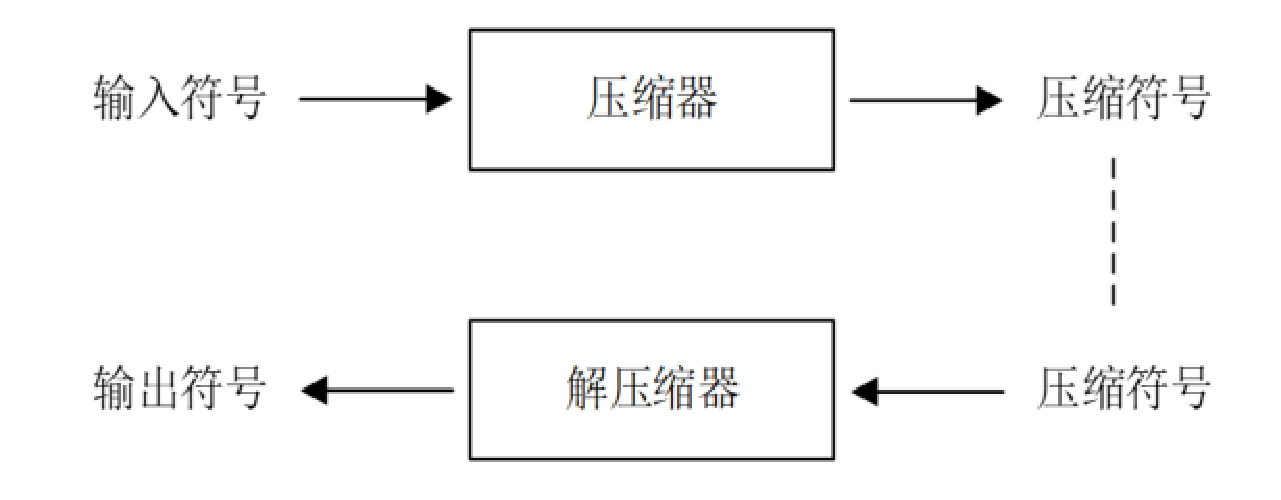
\includegraphics[height=4cm,width=12cm,angle=0,scale=1]{21.eps}
  \caption{压缩通用流程图}\label{25}
     \end{figure}

\subsection{游程编码}

游程编码,又称运行长度编码,指由一连串字符(或信号采样值)组成的数字编码。该编码属于无损压缩编码,其广泛应用于数据压缩领域,同时游程编码\cite{54}也是作为二值图的重要编码方法之一。目前在数据压缩算法中较为常用的游程编码有Golomb 编码\cite{55}、FDR编码\cite{56}、EFDR 编码\cite{57}以及交替游程编码(ALT-FDR)\cite{58}。根据游程编码进行分类,有单游程编码和双游程编码两种方式。其中单游程编码中比较常见的有FDR 编码,FDR 编码的基本规则是,只对游程中 0 的长串进行编码,根据 0 串的长度会生成唯一的码字,当 0 串越长所对应的码字相对于原串而言就越短,从而压缩率也越高,对于游程中出现的 1 比特位,我们使用使用码字 00 来进行编码,因此当测试集中1比特位较多时,不建议使用FDR编码,EFDR的效果更佳。下表
\ref{tabl2}为FDR的前几组编码。

EFDR编码不仅可以使用较短的码字对连续的0码字进行编码,对于连续的1码字也同样适用。当测试集的跳变数越少,使用EFDR编码所能达到的压缩率就越高。下表\ref{tabl3}为EFDR前一部分编码规则。下面举例说明EFDR的的压缩流程。测试向量$T={1111110 0000001 111111111111110}$,根据EFDR码表可将其划分为三个游程,其长度分别为{6,6,14}。使用EFDR编码压缩后测试向量变为{11010 01010 1110111},减少了12位。
\begin{table}[H]
\centering
\caption{FDR编码表}\label{tabl2}
\begin{tabular}{p{1.6cm}p{2.7cm}<{\centering}p{2.7cm}<{\centering}p{3cm}<{\centering}p{3.6cm}<{\centering}}
\toprule
\textbf{组}&	\textbf{游程长度}&     \textbf{前缀}&   \textbf{尾部}&   \textbf{码字}\\
\midrule
\multirow{2}{*}{A1} & 0 & \multirow{2}{*}{0} & 0 & 00 \\
& 1 &  & 1 & 01 \\
\hline
\multirow{4}{*}{A2} & 2 & \multirow{4}{*}{10} & 00 & 1000 \\
& 3 &  & 01 & 1001 \\
& 4 &  & 10 & 1010 \\
& 5 &  & 11 & 1011 \\
\hline
\multirow{8}{*}{A3} & 6 & \multirow{8}{*}{110} & 000 & 110000 \\
& 7 &  & 001 & 110001 \\
& 8 &  & 010 & 110010 \\
& 9 &  & 011 & 110011 \\
& 10 &  & 100 & 110100 \\
& 11 &  & 101 & 110101 \\
& 12 &  & 110 & 110110 \\
& 13 &  & 111 & 110111 \\
\bottomrule
\end{tabular}
\end{table}

\begin{table}[H]
\centering
\caption{EFDR编码表}\label{tabl3}
\begin{tabular}{p{1.6cm}p{1.6cm}<{\centering}p{2.2cm}<{\centering}p{2.2cm}<{\centering}p{3cm}<{\centering}p{3cm}<{\centering}}
\toprule
\textbf{组}&	\textbf{游程长度}&     \textbf{前缀}&   \textbf{尾部}&   \textbf{0油程}&   \textbf{1油程}\\
\midrule
\multirow{2}{*}{A1} & 1 & \multirow{2}{*}{0} & 0 & 000& 100 \\
& 2 &  & 1 & 001 & 101 \\
\hline
\multirow{4}{*}{A2} & 3 & \multirow{4}{*}{10} & 00 & 01000& 11000 \\
& 4 &  & 01 & 01001 & 11001\\
& 5 &  & 10 & 01010 & 11010 \\
& 6 &  & 11 & 01011 & 11011 \\
\hline
\multirow{8}{*}{A3} & 7 & \multirow{8}{*}{110} & 000 & 0110000 & 1110000 \\
& 8 &  & 001 & 0110001 & 1110001 \\
& 9 &  & 010 & 0110010 & 1110010 \\
& 10 &  & 011 & 0110011 & 1110011 \\
& 11 &  & 100 & 0110100 & 1110100 \\
& 12 &  & 101 & 0110101 & 1110101 \\
& 13 &  & 110 & 0110110 & 1110110 \\
& 14 &  & 111 & 0110111 & 1110111 \\
\bottomrule
\end{tabular}
\end{table}

\subsection{字典编码}

字典编码是一种随着数据流本身的特点动态地构建适合该数据流的编码,在文本压缩、音频压缩中应用比较广泛。相比于统计编码,它的实现既不需要用到统计的方法,也不需要用到变长码的方式,而是从数据流中选择多个字符串,利用字典的方式,对其进行编码压缩。字典编码根据是否可以通过静态的方式对数据流中的字符串进行保存分为非自适应LZ编码和自适应LZ编码。

下图\ref{26}是使用完全字典压缩方法的原理图,图中$b$代表测试通道的数量。$n$代表扫描链的数量,$n$的值往往大于$b$,$n$与$b$的比值越大,每一条扫描链的长度就越。使用此方法能提高加载测试向量的效率,减少测试时间。其不足之处在于,若使用完全字典的方式,需要存储巨大的数据量,增大硬件开销。因此部分学者使用部分字典的方式,对不在字典中的数据进行纠错以达到控制字典的大小,通过在硬件代价与纠错成本之间进行权衡,从而达到一定的压缩率。

\begin{figure}[H]
  \centering
  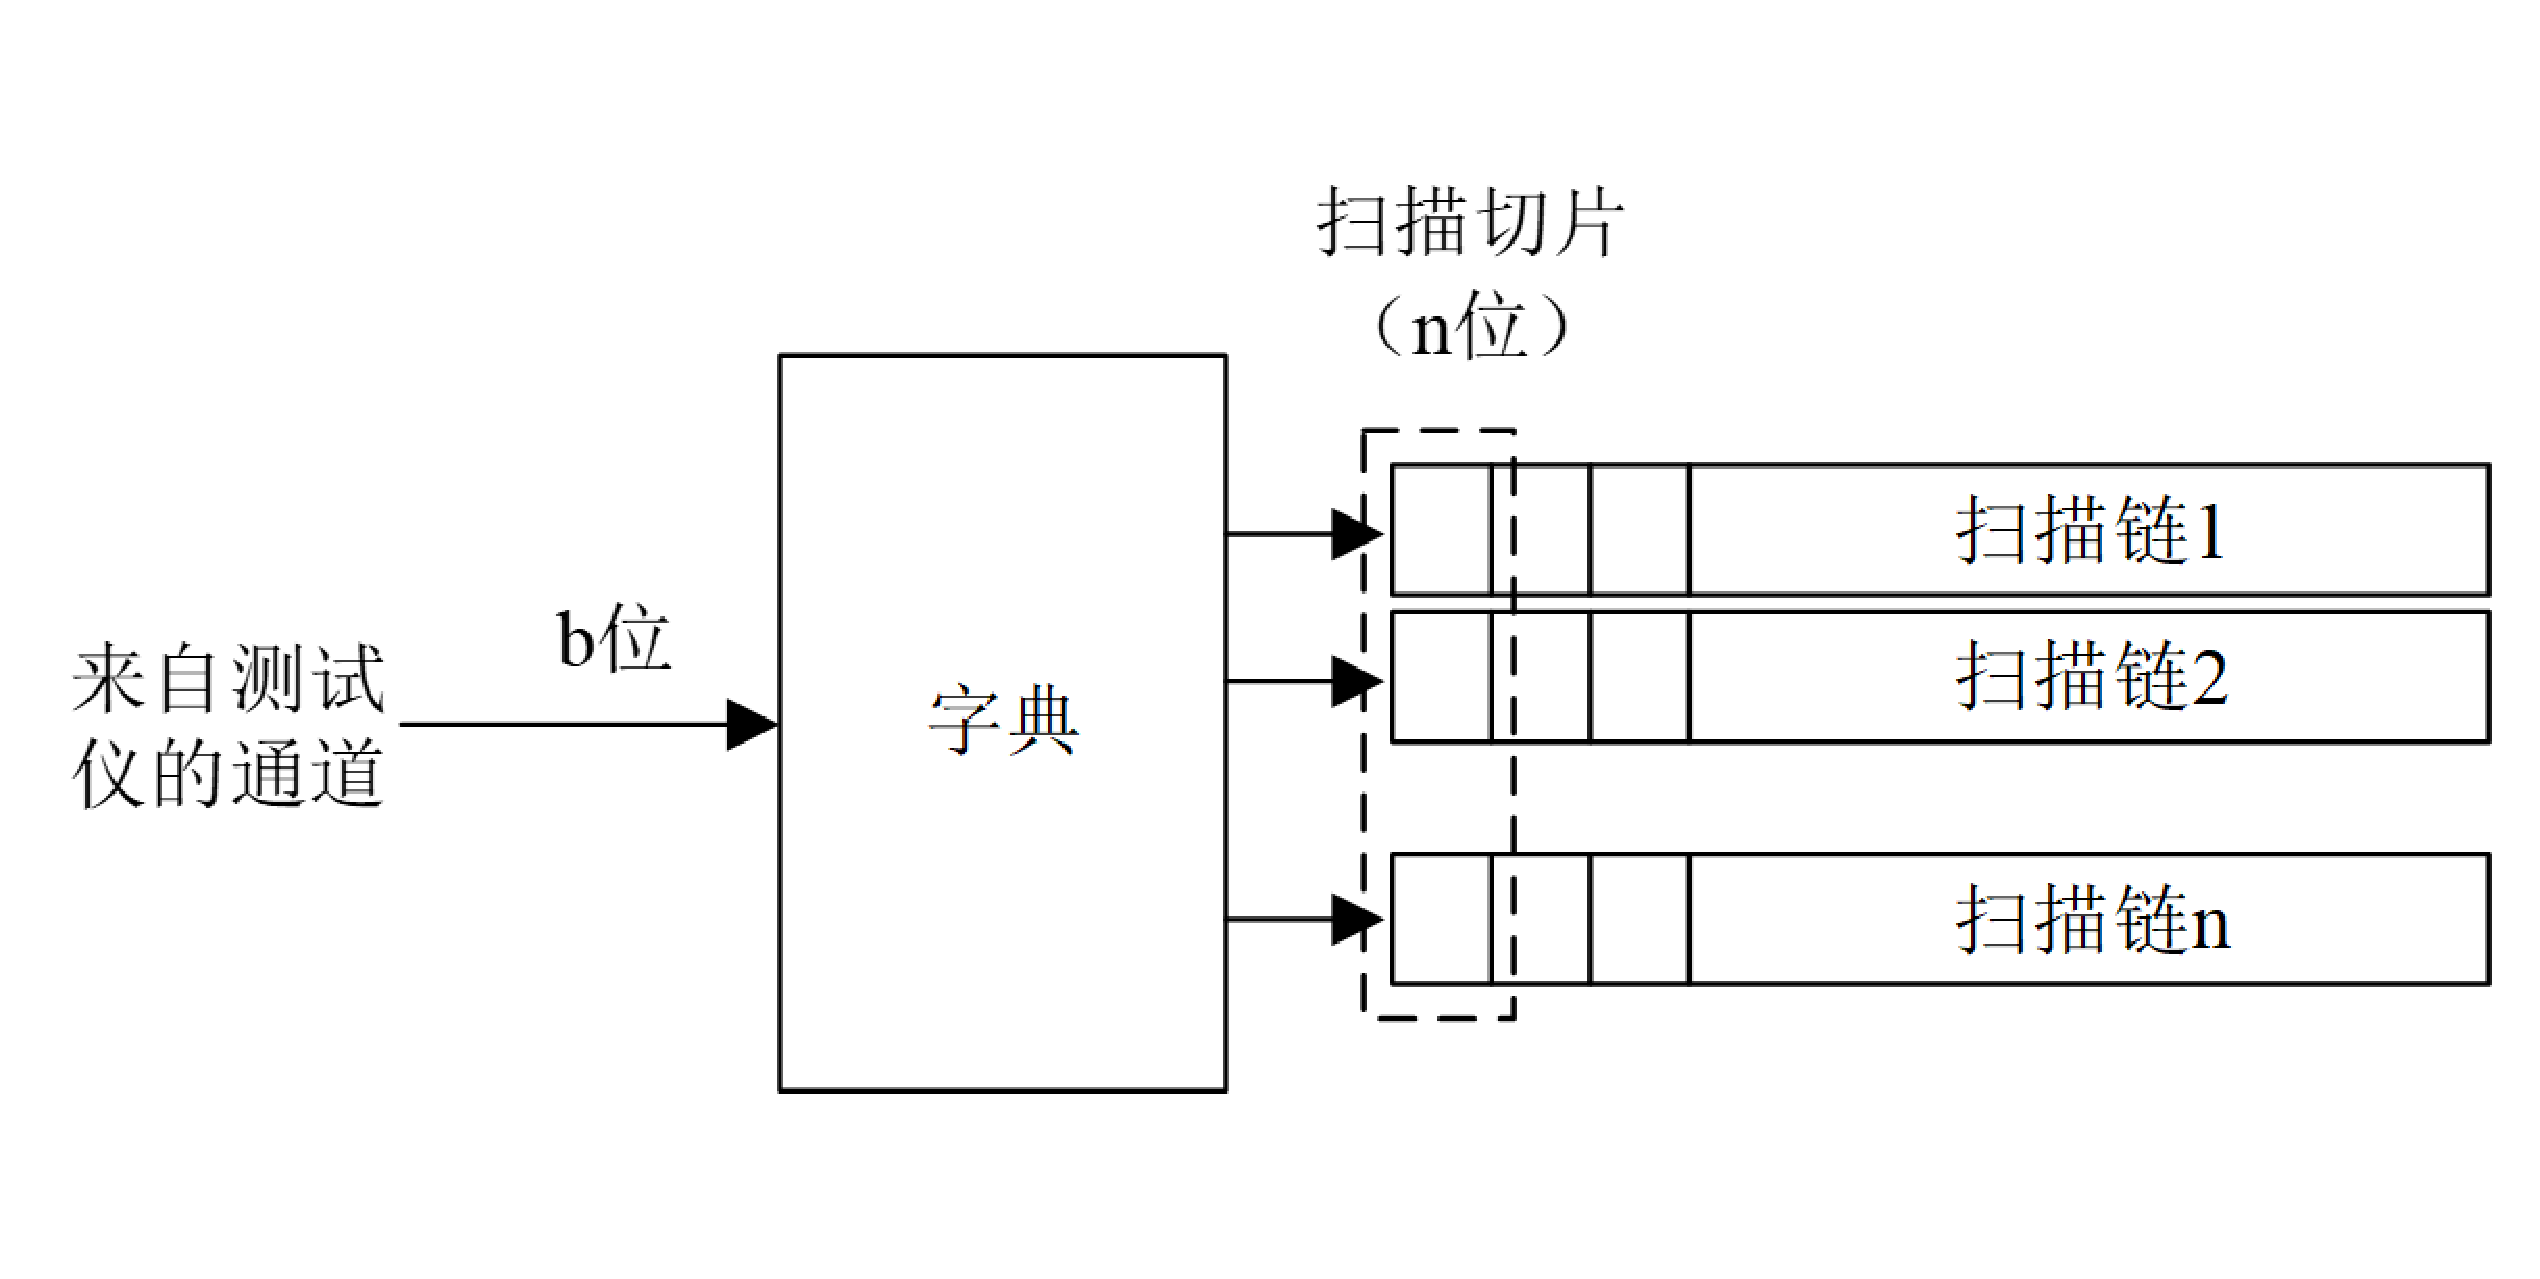
\includegraphics[height=7cm,width=14cm,angle=0,scale=1]{26.eps}
  \caption{字典压缩方法}\label{26}
     \end{figure}

\subsection{统计编码}

统计编码是一种在测试数据压缩中广泛运用的压缩方法。其本质就是通过某种方式将原数据集拆分为一个个数据块并进行数学统计,将重复率高的数据块以短码字编码,从而达到数据压缩的目的。假定原数据集合为$X$,先按照一定的规则对$X$ 进行分块或者分类,统计出相同块 的数量,然后进行编码。被大家广为熟知的有霍夫曼编码\cite{59}。 霍夫曼编码通过构造霍夫曼树,将原数据集合拆分成为等长的信源符号。然后统计出相同的信源符号的个数并排序,将重复次数多的部分用短码字描述,重复次数少的部分用长码字描述,从而减少原测试集中的比特位,压缩测试数据。

部分学者对Huffman编码进行改进,衍生出譬如最优选择哈夫曼(OP-SHC)\cite{60}以及多级哈夫曼\cite{61,62,63}等编码方式。下面将举例说明如何使用霍夫曼编码,下图中框中为本例使用的数据集,总共有80位。对于初始数据集的处理,首先将其划分成为4 位为一组的比特块,然后将每一个比特块出现的频率进行统计,如下表\ref{tabl5} 所示,可以发现表中1010、0000、1111三种数据块出现的频率最高。最后对出现次数最多比特块进行霍夫曼编码,如下图\ref{27}所示。对于未编码的块则需要在原有码字之前加上111,通过使用霍夫曼编码可将原数据集中的数据压缩38.8\%。

\begin{table}[H]
\centering
\caption{测试集的划分和各种块出现的频率}\label{tabl5}
\begin{tabular}{p{7cm}<{\centering}p{2.7cm}<{\centering}p{2.7cm}<{\centering}}
\toprule
\textbf{测试集T}&	\textbf{不同的块}&     \textbf{频率}\\
\midrule
1010 0000 1010 1111 &1010 & 9/20\\
1111 0000 1010 0001	&0000&5/20\\
1010 0000 0010 1010	&1111&3/20\\
0000 1010 1010 0000	&0001&2/20\\
1010 1111 1010 0001	&0010&1/20\\
\bottomrule
\end{tabular}
\end{table}

\begin{figure}[H]
  \centering
  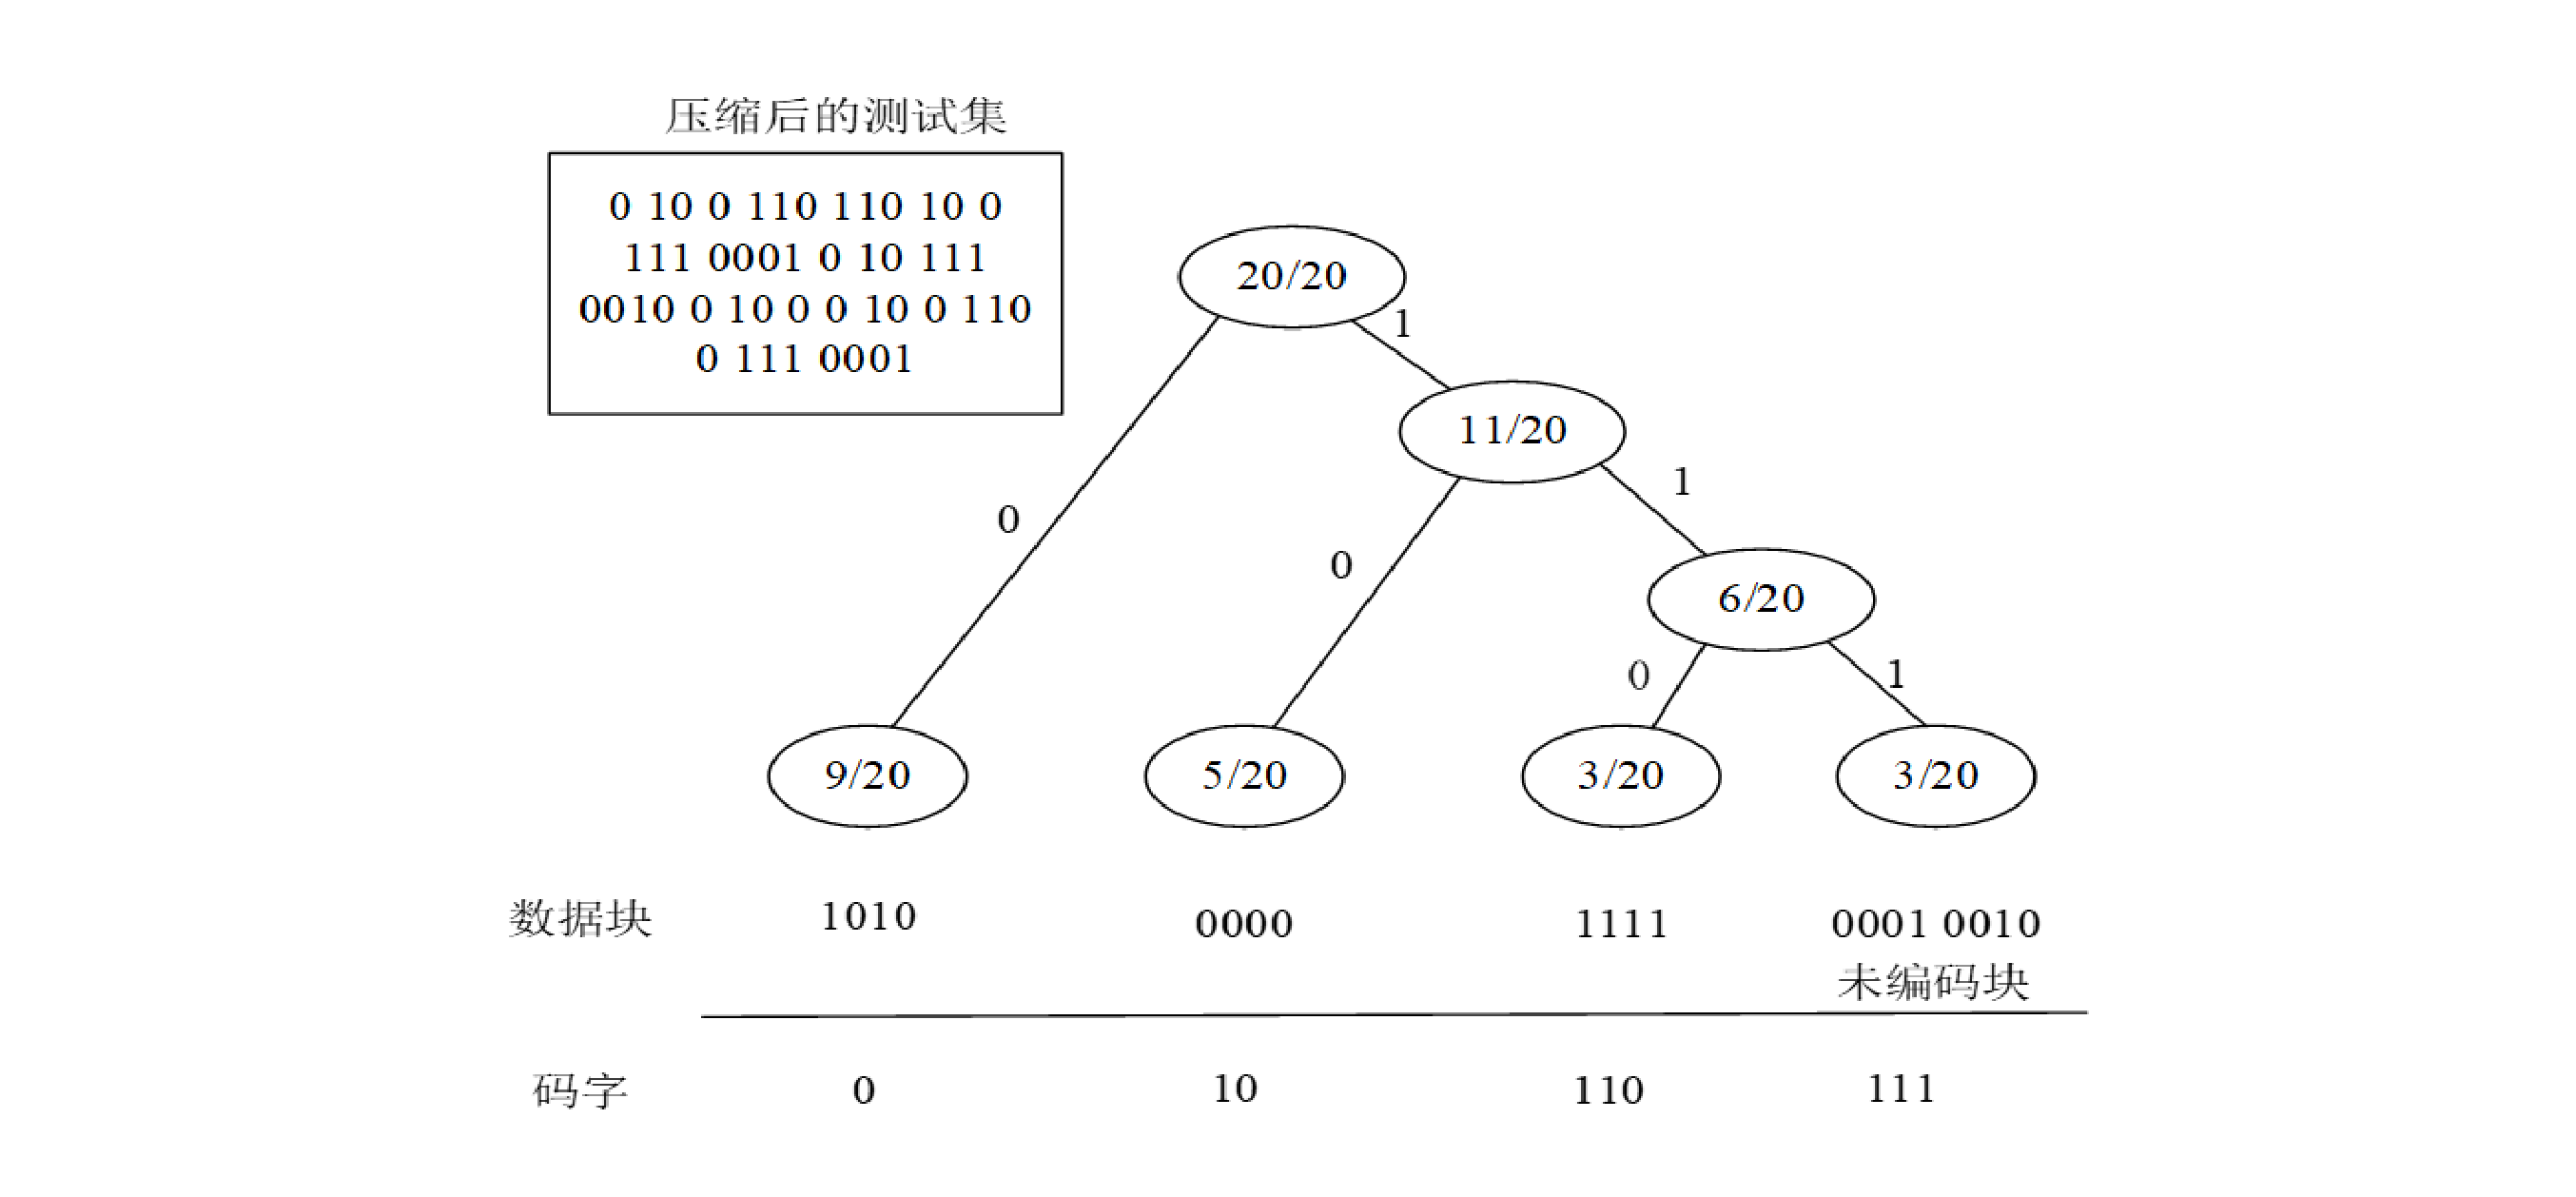
\includegraphics[height=10cm,width=16cm,angle=0,scale=1]{27.eps}
  \caption{最优选择哈夫曼编码}\label{27}
     \end{figure}

除了上文介绍的几种编码外,9C\cite{64}、多层复制\cite{65}、块合并\cite{66}、BM-8C\cite{67}、SVC\cite{68}、 选择扫描切片\cite{69} 等编码在数据压缩领域也较为常用。

\section{非编码压缩}

\subsection{基于线性解压缩}

线性解压缩器是一种包含了D触发器、RS触发器以及异或门的解压缩结构,如下图\ref{28}所示,其由四部分组成,左边是拥有$b$个通道的代码测试仪,经过LFSR到达了组合线性网络,然后将LFSR中的数据扩展至右边的$n$条扫描链中,每一条扫描链中有$m$位数据,因此需要$b(q+m)$ 个比特位的数据才能产生一个测试集。当对测试集解压缩时,线性反馈移位寄存器会将压缩数据还原为原测试集合并进行初始化,等待时钟周期的到来再将数据传送至扫描链。

\begin{figure}[H]
  \vspace{\baselineskip}
  \centering
  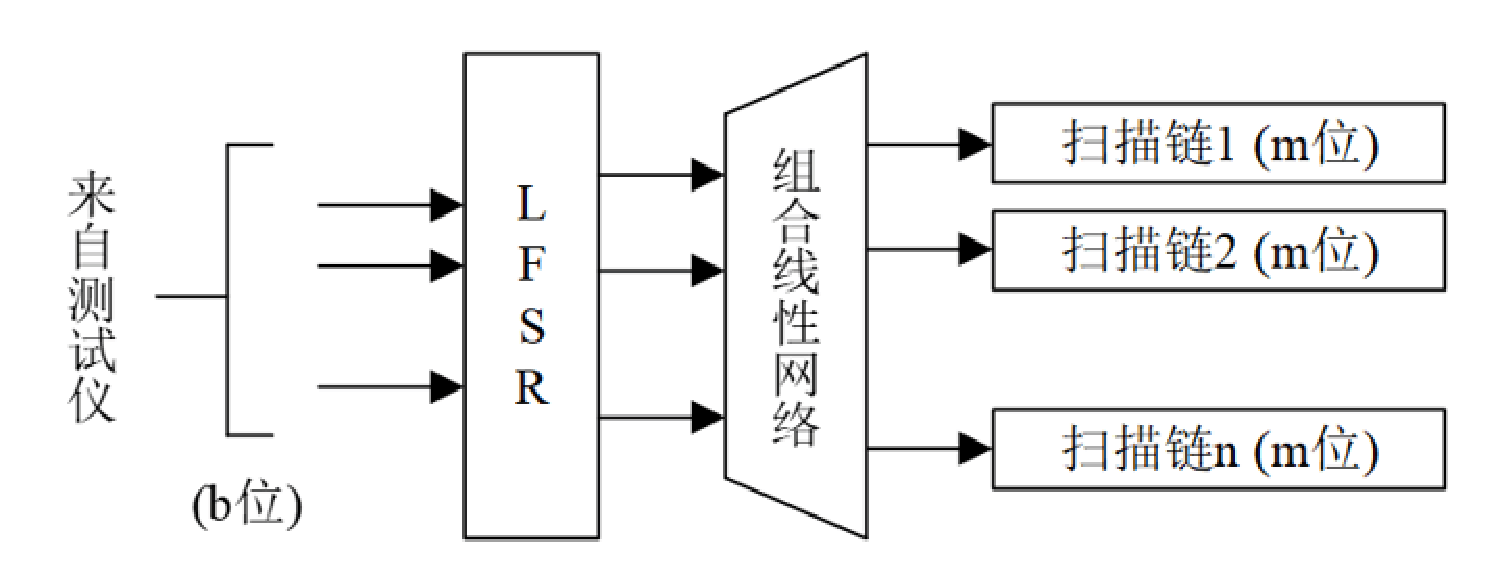
\includegraphics[height=4cm,width=14cm,angle=0,scale=1]{28.eps}
  \vspace{\baselineskip}
  \caption{时序线性解压器}\label{28}
     \end{figure}

\subsection{基于广播扫描}

“广播扫描”从字面上的意思来理解,就是使用广播的方式将数据施加多条扫描链,可以类比于IO多路复用的方式,即使用一个线程监听多个socket, 在本实验中即驱动多个扫描链。其中Illinois扫描结构\cite{70}比较具有代表性,其结构如图\ref{29}所示。

\begin{figure}[H]
  \centering
  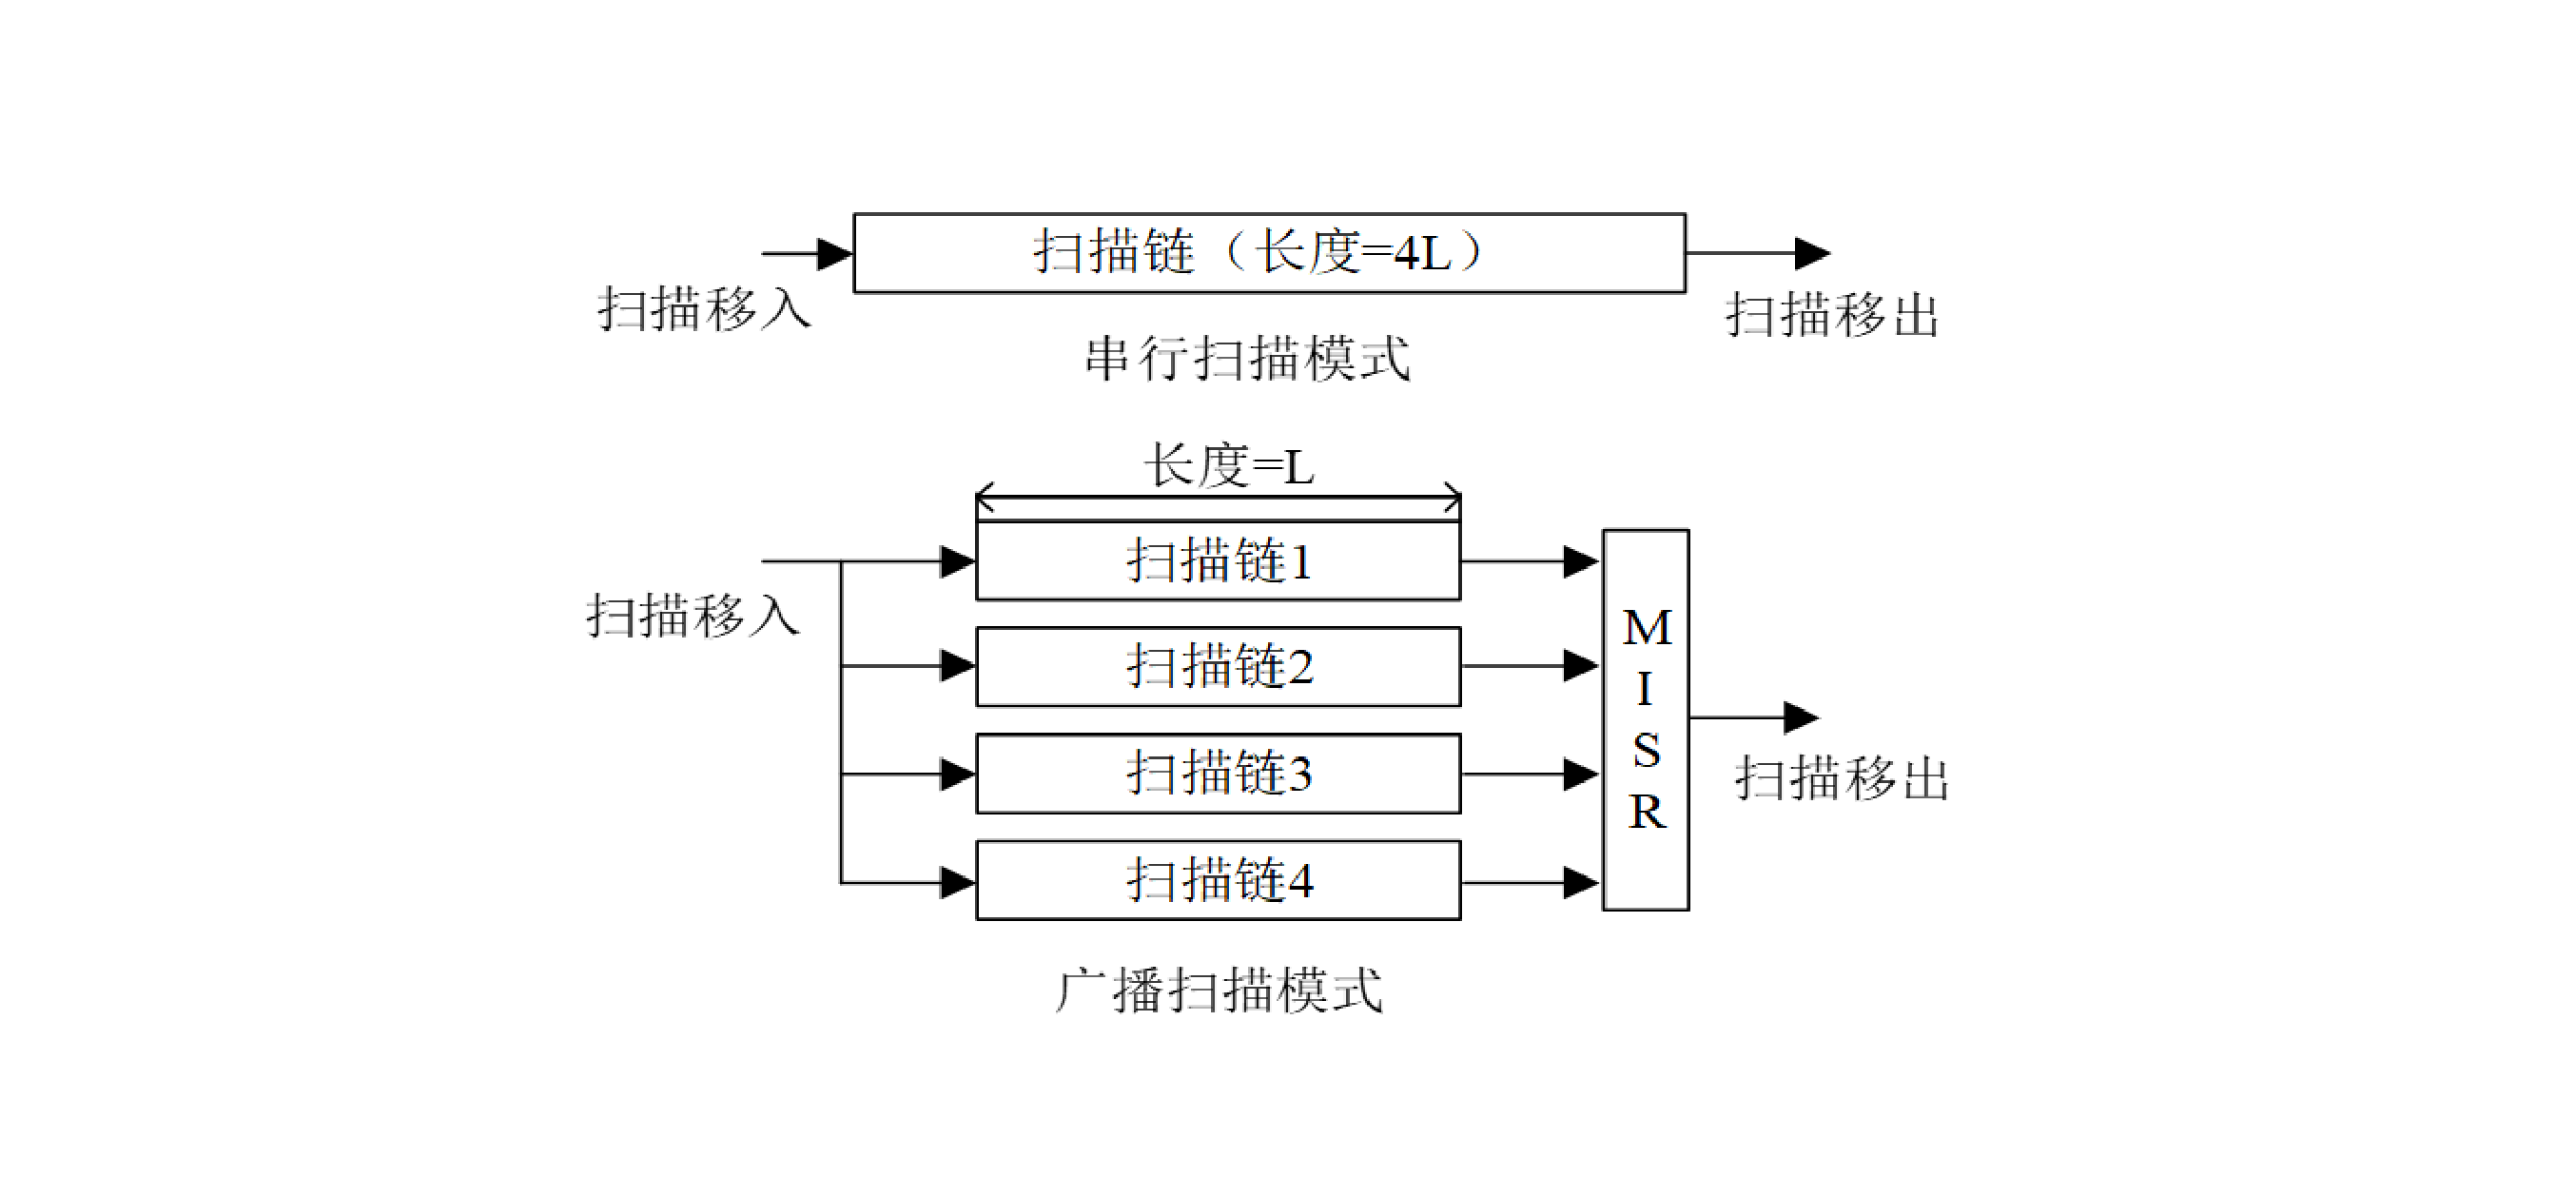
\includegraphics[height=8cm,width=16cm,angle=0,scale=1]{29.eps}
  \caption{广播扫描结构}\label{29}
     \end{figure}

广播扫描模式较传统扫描模式不同点在于,广播扫描模式将扫描链进行拆分并将扫描链连接到同一输入。上图的原始扫描链为$4L$,每一个子扫描链都为$L$,这可能会导致故障遗漏,因此,需要结合串行扫描模式才能排查出电路中存在的故障,提高故障覆盖率。广播扫描模式由于扫描链之间会存在相等值,将导致某些故障无法检测,因此多输入扫描链的方式应运而生。其改进的措施为先将扫描链分为多组,每一组的输入端均不相同但组内数据相容,最终确保每一组故障覆盖率达标。 其次采取重新配置广播扫描链的结构或者降低测试过程所需的功耗也可用来提高压缩率。

\section{哈达码变换}

\subsection{基本原理}

哈达码变换是利用哈达码矩阵作为变换矩阵,将原有数据表示为新数据的一种变换方式。自然界有很多的信号,例如图像、声音、视频等经过变换编码后进行高倍率的压缩。哈达码变换使用通式$Y=HX$ 表示,其中 $X$ 和 $Y$ 均是一列向量,$H$ 为哈达码矩阵。哈达码变换已广泛应用于视频和音频编码中,由于其硬件代价低实现简单的特点,也被人们应用于测试数据压缩。与多媒体数据的压缩的不同之处是,激励压缩属于无损压缩。

\subsection{哈达码矩阵以及变换的基本流程}

哈达码变换中使用的矩阵由-1和1组成,这种天然的特性非常适用于电路测试,矩阵中1等价于测试集中的1比特位,-1等价于测试集中的0 比特位。哈达码矩阵可以被递归定义:

\begin{equation}
H(k)
=
\left[
\begin{array}{cc}
    H(k-1)&H(k-1)\\
    H(k-1)&-H(k-1)\\
\end{array}
\right]
,k=1,2,....,n,
\end{equation}

其中H(0)=1,根据上述通式,当$k=1$以及$k=2$时有下列矩阵:

\begin{equation}
H(1)
=
\left[
\begin{array}{cc}
    1&1\\
    1&-1\\
\end{array}
\right]
\end{equation}

\begin{equation}
H(2)
=
\left[
\begin{array}{cccc}
    1&1&1&1\\
    1&-1&1&-1\\
    1&1&-1&-1\\
    1&-1&-1&1\\
\end{array}
\right]
\end{equation}

哈达码矩阵的行列均是一个基本向量,本文将其称作Walsh函数。以 H(2)为例,它有 4 个基本向量,通过向量间两两相互组合,就可以变换出任何一个具有4个比特位的列向量。比如向量[4 -4 -2 -4]可以被写为-1$\ast$[2 2 2 2]+1$\ast$[2 -2 2 -2] +1$\ast$[2 2 -2 -2] +1$\ast$[2 -2 -2 2]。基于此,电路的测试集均可以通过使用一组Walsh函数表示。

下面具体介绍一下如何使用哈达码矩阵进行拆分压缩的变换,首先根据原测试集的大小确定需要递归迭代的次数,然后对原测试集中的某一列用 WHT 变换提取主分量,实质就是从哈达码矩阵中选取最合适的Walsh 函数来近似代替这一列。也就是说,通过将当前列向量与所有的 Walsh 函数进行比较,选取差异最小的那一个 Walsh 函数作为主分量。依次以原测试集中每一列为基准找出相对应的主分量构成主分量集,从上文分析可知,向量分解对单游程编码最有效,因为在变换中实验每次都是选取使得残分量中 1 最少的 Walsh 函数作为主分量。然而,对于双游程编码(EFDR、RL-Huff、ALT-FDR)、分块编码(OP-SHC)等方法而言,减少测试集中的 1 并不是最优策略。

\subsection{哈达码变换的优缺点}

实验结果表明哈达码变换取得了较好的压缩收益,其主要优点有两个,第一哈达码矩阵通过递归调用之后生成全新矩阵,所涉及的硬件代价开销小。第二,通过递归最终生成的矩阵中,所有列向量两两之间均有差异,与原测试集中列向量匹配概率随之增大,最后得到残差集中0比特位也会更多。

哈达码矩阵中的列向量是随机的,是无特征的状态,有可能与原测试集中列向量差距较大,若哈达码矩阵中的列向量取自原测试集合,原则上来讲会取得更高的压缩增益,本文就是基于这一点展开的研究。

\subsection{使用聚类思想构造主分量集合}

哈达码矩阵中的列向量并非取自原测试集合,若对原测试集进行聚类,选取聚类中心作为基向量,生成主分量集合是否可以提高压缩增益。其中涉及到三个需要解决的问题,第一:原测试集合中存在较多的无关位,对于存在无关位的向量如何进行聚类。第二:原测试集的聚类中心无法确定,由于硬件存储开销,基向量的选取的个数需要符合一定的条件,不可能完全覆盖原测试集合,本实验中基向量选取的个数$k=log2n$其中$n$为原测试集的行数。第三:如何通过$k$列基向量生成大量的列向量,并产生具有更高压缩增益的主分量集合。下文将对三个问题逐一提供解决方案。

\section{小结}

本章详细阐述超大规模集成电路测试相关的概念、原理以及常用的压缩方法。首先本章对测试压缩原理进行了简要的描述。其次,重点介绍了编码压缩,对FDR编码、EFDR编码、Huffman编码逐一举例分析其压缩原理,以及压缩特点。除了编码压缩,也提及了基于非编码的压缩方法。由于本文的研究主要是基于拆分压缩,并且是与哈达码变换进行对比,因此详细介绍了相关知识。其中包括哈达码矩阵的构造、哈达码变换的基本流程以及哈达码变换存在的优势以及不足,最后提出了使用聚类方法构造主分量集合这一思想。


